% Options for packages loaded elsewhere
\PassOptionsToPackage{unicode}{hyperref}
\PassOptionsToPackage{hyphens}{url}
%
\documentclass[
]{article}
\usepackage{lmodern}
\usepackage{amsmath}
\usepackage{ifxetex,ifluatex}
\ifnum 0\ifxetex 1\fi\ifluatex 1\fi=0 % if pdftex
  \usepackage[T1]{fontenc}
  \usepackage[utf8]{inputenc}
  \usepackage{textcomp} % provide euro and other symbols
  \usepackage{amssymb}
\else % if luatex or xetex
  \usepackage{unicode-math}
  \defaultfontfeatures{Scale=MatchLowercase}
  \defaultfontfeatures[\rmfamily]{Ligatures=TeX,Scale=1}
\fi
% Use upquote if available, for straight quotes in verbatim environments
\IfFileExists{upquote.sty}{\usepackage{upquote}}{}
\IfFileExists{microtype.sty}{% use microtype if available
  \usepackage[]{microtype}
  \UseMicrotypeSet[protrusion]{basicmath} % disable protrusion for tt fonts
}{}
\makeatletter
\@ifundefined{KOMAClassName}{% if non-KOMA class
  \IfFileExists{parskip.sty}{%
    \usepackage{parskip}
  }{% else
    \setlength{\parindent}{0pt}
    \setlength{\parskip}{6pt plus 2pt minus 1pt}}
}{% if KOMA class
  \KOMAoptions{parskip=half}}
\makeatother
\usepackage{xcolor}
\IfFileExists{xurl.sty}{\usepackage{xurl}}{} % add URL line breaks if available
\IfFileExists{bookmark.sty}{\usepackage{bookmark}}{\usepackage{hyperref}}
\hypersetup{
  pdftitle={Patterson\_Lab8},
  pdfauthor={Tim Patterson},
  hidelinks,
  pdfcreator={LaTeX via pandoc}}
\urlstyle{same} % disable monospaced font for URLs
\usepackage[margin=1in]{geometry}
\usepackage{color}
\usepackage{fancyvrb}
\newcommand{\VerbBar}{|}
\newcommand{\VERB}{\Verb[commandchars=\\\{\}]}
\DefineVerbatimEnvironment{Highlighting}{Verbatim}{commandchars=\\\{\}}
% Add ',fontsize=\small' for more characters per line
\usepackage{framed}
\definecolor{shadecolor}{RGB}{248,248,248}
\newenvironment{Shaded}{\begin{snugshade}}{\end{snugshade}}
\newcommand{\AlertTok}[1]{\textcolor[rgb]{0.94,0.16,0.16}{#1}}
\newcommand{\AnnotationTok}[1]{\textcolor[rgb]{0.56,0.35,0.01}{\textbf{\textit{#1}}}}
\newcommand{\AttributeTok}[1]{\textcolor[rgb]{0.77,0.63,0.00}{#1}}
\newcommand{\BaseNTok}[1]{\textcolor[rgb]{0.00,0.00,0.81}{#1}}
\newcommand{\BuiltInTok}[1]{#1}
\newcommand{\CharTok}[1]{\textcolor[rgb]{0.31,0.60,0.02}{#1}}
\newcommand{\CommentTok}[1]{\textcolor[rgb]{0.56,0.35,0.01}{\textit{#1}}}
\newcommand{\CommentVarTok}[1]{\textcolor[rgb]{0.56,0.35,0.01}{\textbf{\textit{#1}}}}
\newcommand{\ConstantTok}[1]{\textcolor[rgb]{0.00,0.00,0.00}{#1}}
\newcommand{\ControlFlowTok}[1]{\textcolor[rgb]{0.13,0.29,0.53}{\textbf{#1}}}
\newcommand{\DataTypeTok}[1]{\textcolor[rgb]{0.13,0.29,0.53}{#1}}
\newcommand{\DecValTok}[1]{\textcolor[rgb]{0.00,0.00,0.81}{#1}}
\newcommand{\DocumentationTok}[1]{\textcolor[rgb]{0.56,0.35,0.01}{\textbf{\textit{#1}}}}
\newcommand{\ErrorTok}[1]{\textcolor[rgb]{0.64,0.00,0.00}{\textbf{#1}}}
\newcommand{\ExtensionTok}[1]{#1}
\newcommand{\FloatTok}[1]{\textcolor[rgb]{0.00,0.00,0.81}{#1}}
\newcommand{\FunctionTok}[1]{\textcolor[rgb]{0.00,0.00,0.00}{#1}}
\newcommand{\ImportTok}[1]{#1}
\newcommand{\InformationTok}[1]{\textcolor[rgb]{0.56,0.35,0.01}{\textbf{\textit{#1}}}}
\newcommand{\KeywordTok}[1]{\textcolor[rgb]{0.13,0.29,0.53}{\textbf{#1}}}
\newcommand{\NormalTok}[1]{#1}
\newcommand{\OperatorTok}[1]{\textcolor[rgb]{0.81,0.36,0.00}{\textbf{#1}}}
\newcommand{\OtherTok}[1]{\textcolor[rgb]{0.56,0.35,0.01}{#1}}
\newcommand{\PreprocessorTok}[1]{\textcolor[rgb]{0.56,0.35,0.01}{\textit{#1}}}
\newcommand{\RegionMarkerTok}[1]{#1}
\newcommand{\SpecialCharTok}[1]{\textcolor[rgb]{0.00,0.00,0.00}{#1}}
\newcommand{\SpecialStringTok}[1]{\textcolor[rgb]{0.31,0.60,0.02}{#1}}
\newcommand{\StringTok}[1]{\textcolor[rgb]{0.31,0.60,0.02}{#1}}
\newcommand{\VariableTok}[1]{\textcolor[rgb]{0.00,0.00,0.00}{#1}}
\newcommand{\VerbatimStringTok}[1]{\textcolor[rgb]{0.31,0.60,0.02}{#1}}
\newcommand{\WarningTok}[1]{\textcolor[rgb]{0.56,0.35,0.01}{\textbf{\textit{#1}}}}
\usepackage{graphicx}
\makeatletter
\def\maxwidth{\ifdim\Gin@nat@width>\linewidth\linewidth\else\Gin@nat@width\fi}
\def\maxheight{\ifdim\Gin@nat@height>\textheight\textheight\else\Gin@nat@height\fi}
\makeatother
% Scale images if necessary, so that they will not overflow the page
% margins by default, and it is still possible to overwrite the defaults
% using explicit options in \includegraphics[width, height, ...]{}
\setkeys{Gin}{width=\maxwidth,height=\maxheight,keepaspectratio}
% Set default figure placement to htbp
\makeatletter
\def\fps@figure{htbp}
\makeatother
\setlength{\emergencystretch}{3em} % prevent overfull lines
\providecommand{\tightlist}{%
  \setlength{\itemsep}{0pt}\setlength{\parskip}{0pt}}
\setcounter{secnumdepth}{-\maxdimen} % remove section numbering
\ifluatex
  \usepackage{selnolig}  % disable illegal ligatures
\fi

\title{Patterson\_Lab8}
\author{Tim Patterson}
\date{04/28/2021}

\begin{document}
\maketitle

\textbf{1. Use \texttt{tidycensus} to download 1. race/ethnicity
(B03002) and 2. median household income for Baltimore City. Store this
data in a new object. Choose which race/ethnicity you'd like to relate
to income (Non-Hispanic Black and Non-Hispanic White work best). Which
census tract has the highest \emph{percentage} of your target
race/ethnicity (and what is the percent) and which has the highest
median household income (and how much is it?)? (5 points)} Reminder:
Since we will be mapping our data, make sure you include use
\texttt{geometry\ =\ TRUE} in \texttt{get\_acs()}

\begin{Shaded}
\begin{Highlighting}[]
\CommentTok{\# settings for tidycensus}
\FunctionTok{options}\NormalTok{(}\AttributeTok{tigris\_class =} \StringTok{"sf"}\NormalTok{)}
\FunctionTok{options}\NormalTok{(}\AttributeTok{tigris\_use\_cache =} \ConstantTok{TRUE}\NormalTok{)}
\FunctionTok{census\_api\_key}\NormalTok{(}\StringTok{"7da13c910d6b0d231eff70a1168b636ee281edd3"}\NormalTok{, }\AttributeTok{overwrite =} \ConstantTok{TRUE}\NormalTok{)}
\end{Highlighting}
\end{Shaded}

\begin{verbatim}
## To install your API key for use in future sessions, run this function with `install = TRUE`.
\end{verbatim}

\begin{Shaded}
\begin{Highlighting}[]
\FunctionTok{setwd}\NormalTok{(}\StringTok{"C:/Users/vival/Documents/GES 486/Lab8"}\NormalTok{)}


\CommentTok{\# This gets African American Population and MHHI in 2019}
\NormalTok{MD\_household\_2019 }\OtherTok{\textless{}{-}} \FunctionTok{get\_acs}\NormalTok{(}\AttributeTok{geography =} \StringTok{"tract"}\NormalTok{, }
     \AttributeTok{variables =} \FunctionTok{c}\NormalTok{(}\StringTok{"total\_population"} \OtherTok{=} \StringTok{"B01003\_001"}\NormalTok{, }\CommentTok{\# Total population}
                   \StringTok{"black\_pop"} \OtherTok{=} \StringTok{"B01001B\_001"}\NormalTok{,}
                   \StringTok{"med\_hh\_inc"} \OtherTok{=} \StringTok{"B19013\_001"} \CommentTok{\# Median household income}
\NormalTok{                   ), }
     \AttributeTok{year =} \DecValTok{2019}\NormalTok{,}
     \AttributeTok{survey =} \StringTok{"acs5"}\NormalTok{,}
     \AttributeTok{state =} \FunctionTok{c}\NormalTok{(}\DecValTok{24}\NormalTok{), }
     \AttributeTok{county =} \FunctionTok{c}\NormalTok{(}\DecValTok{510}\NormalTok{),}
     \AttributeTok{geometry =} \ConstantTok{TRUE}\NormalTok{, }\CommentTok{\# download the shapefile with the data}
     \AttributeTok{output =} \StringTok{"wide"}\NormalTok{)}\SpecialCharTok{\%\textgreater{}\%} \FunctionTok{clean\_names}\NormalTok{() }\CommentTok{\# need this 2019}
\end{Highlighting}
\end{Shaded}

\begin{verbatim}
## Getting data from the 2015-2019 5-year ACS
\end{verbatim}

\begin{Shaded}
\begin{Highlighting}[]
\NormalTok{MD\_household\_2019}\SpecialCharTok{$}\NormalTok{blackprop }\OtherTok{=}\NormalTok{ MD\_household\_2019}\SpecialCharTok{$}\NormalTok{black\_pop\_e }\SpecialCharTok{/} 
\NormalTok{MD\_household\_2019}\SpecialCharTok{$}\NormalTok{total\_population\_e}
\FunctionTok{max}\NormalTok{(MD\_household\_2019}\SpecialCharTok{$}\NormalTok{black\_pop\_e)}
\end{Highlighting}
\end{Shaded}

\begin{verbatim}
## [1] 7141
\end{verbatim}

\begin{Shaded}
\begin{Highlighting}[]
\NormalTok{baltdrop2 }\OtherTok{=}\NormalTok{ MD\_household\_2019}\SpecialCharTok{$}\NormalTok{blackprop[}\SpecialCharTok{!}\FunctionTok{is.na}\NormalTok{(MD\_household\_2019}\SpecialCharTok{$}\NormalTok{blackprop)]}
\FunctionTok{max}\NormalTok{(baltdrop2)}
\end{Highlighting}
\end{Shaded}

\begin{verbatim}
## [1] 0.9931774
\end{verbatim}

\begin{Shaded}
\begin{Highlighting}[]
\NormalTok{baltdata1 }\OtherTok{=}\NormalTok{ MD\_household\_2019 }\SpecialCharTok{\%\textgreater{}\%} \FunctionTok{filter}\NormalTok{(}\SpecialCharTok{!}\FunctionTok{is.na}\NormalTok{(MD\_household\_2019}\SpecialCharTok{$}\NormalTok{med\_hh\_inc\_e))}

\FunctionTok{max}\NormalTok{(baltdata1}\SpecialCharTok{$}\NormalTok{med\_hh\_inc\_e)}
\end{Highlighting}
\end{Shaded}

\begin{verbatim}
## [1] 195156
\end{verbatim}

Census tract 2711.02 gave me the highest median household income with an
amount of \$195,156. Census Tract 2007.02 gave me the highest Percentage
of African Americans with 99.3 \%.

\textbf{2. Please reproject this data to Web Mercator. (1 points)}

\begin{Shaded}
\begin{Highlighting}[]
\NormalTok{baltdata1transform }\OtherTok{=} \FunctionTok{st\_transform}\NormalTok{(baltdata1, }\DecValTok{3857}\NormalTok{)}
\end{Highlighting}
\end{Shaded}

\textbf{3. Create two plots. In the first plot highlight the tract with
the highest concentration of your selected race/eth. In the second plot
highlight the tract with the highest median household income? (5
points)}

\begin{Shaded}
\begin{Highlighting}[]
\FunctionTok{colnames}\NormalTok{(baltdata1)}
\end{Highlighting}
\end{Shaded}

\begin{verbatim}
##  [1] "geoid"              "name"               "total_population_e"
##  [4] "total_population_m" "black_pop_e"        "black_pop_m"       
##  [7] "med_hh_inc_e"       "med_hh_inc_m"       "geometry"          
## [10] "blackprop"
\end{verbatim}

\begin{Shaded}
\begin{Highlighting}[]
\NormalTok{bidata }\OtherTok{=} \FunctionTok{bi\_class}\NormalTok{(baltdata1, }\AttributeTok{x =}\NormalTok{ blackprop, }\AttributeTok{y=}\NormalTok{ med\_hh\_inc\_e, }\AttributeTok{style =} \StringTok{"quantile"}\NormalTok{, }\AttributeTok{dim =} \DecValTok{3}\NormalTok{)}

\NormalTok{highest\_black }\OtherTok{=}\NormalTok{ baltdata1 }\SpecialCharTok{\%\textgreater{}\%} \FunctionTok{filter}\NormalTok{(med\_hh\_inc\_e }\SpecialCharTok{==} \DecValTok{195156}\NormalTok{)}
\NormalTok{highest\_mhhi }\OtherTok{=}\NormalTok{ baltdata1 }\SpecialCharTok{\%\textgreater{}\%} \FunctionTok{filter}\NormalTok{(blackprop }\SpecialCharTok{\textgreater{}} \FloatTok{0.99}\NormalTok{)}

\CommentTok{\# Mapping Highest Percentage of African Americans of Baltimore City}
\FunctionTok{ggplot}\NormalTok{(bidata)}\SpecialCharTok{+}
  \FunctionTok{geom\_sf}\NormalTok{(}\AttributeTok{mapping =} \FunctionTok{aes}\NormalTok{(}\AttributeTok{fill =}\NormalTok{ bi\_class), }\AttributeTok{color =} \StringTok{"white"}\NormalTok{, }\AttributeTok{size =} \FloatTok{0.1}\NormalTok{, }\AttributeTok{show.legend =} \ConstantTok{FALSE}\NormalTok{)}\SpecialCharTok{+}
  \FunctionTok{bi\_scale\_fill}\NormalTok{(}\AttributeTok{pal =} \StringTok{"DkBlue"}\NormalTok{, }\AttributeTok{dim =} \DecValTok{3}\NormalTok{)}\SpecialCharTok{+}
  \FunctionTok{geom\_sf}\NormalTok{(}\AttributeTok{data =}\NormalTok{ highest\_black , }\AttributeTok{fill =} \StringTok{"red"}\NormalTok{, }\AttributeTok{color =} \ConstantTok{NA}\NormalTok{)}\SpecialCharTok{+} \CommentTok{\# Highest Percentage of A.A. displayed in red}
  \FunctionTok{labs}\NormalTok{(}
    \AttributeTok{title =} \StringTok{"Highest Proportion of African American"}\NormalTok{,}
    \AttributeTok{subtitle =} \StringTok{"Baltimore City"}\NormalTok{)}\SpecialCharTok{+}
  \FunctionTok{bi\_theme}\NormalTok{()}
\end{Highlighting}
\end{Shaded}

\includegraphics{Patterson_Lab8_files/figure-latex/unnamed-chunk-4-1.pdf}

\begin{Shaded}
\begin{Highlighting}[]
\CommentTok{\# Mapping Highest Median Household Income of Baltimore City}
\FunctionTok{ggplot}\NormalTok{(bidata)}\SpecialCharTok{+}
  \FunctionTok{geom\_sf}\NormalTok{(}\AttributeTok{mapping =} \FunctionTok{aes}\NormalTok{(}\AttributeTok{fill =}\NormalTok{ bi\_class), }\AttributeTok{color =} \StringTok{"white"}\NormalTok{, }\AttributeTok{size =} \FloatTok{0.1}\NormalTok{, }\AttributeTok{show.legend =} \ConstantTok{FALSE}\NormalTok{)}\SpecialCharTok{+}
  \FunctionTok{bi\_scale\_fill}\NormalTok{(}\AttributeTok{pal =} \StringTok{"DkBlue"}\NormalTok{, }\AttributeTok{dim =} \DecValTok{3}\NormalTok{)}\SpecialCharTok{+}
  \FunctionTok{geom\_sf}\NormalTok{(}\AttributeTok{data =}\NormalTok{ highest\_mhhi , }\AttributeTok{fill =} \StringTok{"red"}\NormalTok{, }\AttributeTok{color =} \ConstantTok{NA}\NormalTok{)}\SpecialCharTok{+} \CommentTok{\# Highest Median Household Income displayed in red}
  \FunctionTok{labs}\NormalTok{(}
    \AttributeTok{title =} \StringTok{"Highest Median Household Income"}\NormalTok{,}
    \AttributeTok{subtitle =} \StringTok{"Baltimore City"}\NormalTok{)}\SpecialCharTok{+}
  \FunctionTok{bi\_theme}\NormalTok{()}
\end{Highlighting}
\end{Shaded}

\includegraphics{Patterson_Lab8_files/figure-latex/unnamed-chunk-5-1.pdf}

\textbf{4. Create a third column using the bi\_class function from the
tutorial. (2 points)}

\begin{Shaded}
\begin{Highlighting}[]
\FunctionTok{colnames}\NormalTok{(baltdata1)}
\end{Highlighting}
\end{Shaded}

\begin{verbatim}
##  [1] "geoid"              "name"               "total_population_e"
##  [4] "total_population_m" "black_pop_e"        "black_pop_m"       
##  [7] "med_hh_inc_e"       "med_hh_inc_m"       "geometry"          
## [10] "blackprop"
\end{verbatim}

\begin{Shaded}
\begin{Highlighting}[]
\CommentTok{\#Creating a third column using the bi\_class function}
\NormalTok{bidata }\OtherTok{=} \FunctionTok{bi\_class}\NormalTok{(baltdata1, }\AttributeTok{x=}\NormalTok{ blackprop, }\AttributeTok{y =}\NormalTok{ med\_hh\_inc\_e, }\AttributeTok{style =} \StringTok{"quantile"}\NormalTok{, }\AttributeTok{dim =} \DecValTok{3}\NormalTok{)}
\end{Highlighting}
\end{Shaded}

\textbf{5. Create a bivariate map with your data. (3 points)}

\begin{Shaded}
\begin{Highlighting}[]
\CommentTok{\# Creating Bi{-}Variate Map}
\NormalTok{bi\_map }\OtherTok{=}
  \FunctionTok{ggplot}\NormalTok{()}\SpecialCharTok{+}
  \FunctionTok{geom\_sf}\NormalTok{(}\AttributeTok{data =}\NormalTok{ bidata, }\AttributeTok{mapping =} \FunctionTok{aes}\NormalTok{(}\AttributeTok{fill =}\NormalTok{ bi\_class), }\AttributeTok{color =} \StringTok{"white"}\NormalTok{, }\AttributeTok{size =} \FloatTok{0.1}\NormalTok{, }\AttributeTok{show.legend =} \ConstantTok{FALSE}\NormalTok{) }\SpecialCharTok{+}
  \FunctionTok{bi\_scale\_fill}\NormalTok{(}\AttributeTok{pal =} \StringTok{"DkBlue"}\NormalTok{, }\AttributeTok{dim =} \DecValTok{3}\NormalTok{)}\SpecialCharTok{+}
  \FunctionTok{labs}\NormalTok{(}
    \AttributeTok{title =} \StringTok{"Proportion of Income and Race"}\NormalTok{, }
    \AttributeTok{subtitle =} \StringTok{"Batimore City"}\NormalTok{)}\SpecialCharTok{+}
  \FunctionTok{bi\_theme}\NormalTok{()}
\end{Highlighting}
\end{Shaded}

\textbf{6. Use the cowplot package and ggdraw, like in the tutorial to
add a legend (2 points)}.

\begin{Shaded}
\begin{Highlighting}[]
\CommentTok{\# Creating bivariate legend using cowplot}
\NormalTok{legend }\OtherTok{\textless{}{-}} \FunctionTok{bi\_legend}\NormalTok{(}\AttributeTok{pal =} \StringTok{"DkBlue"}\NormalTok{,}
                    \AttributeTok{dim =} \DecValTok{3}\NormalTok{,}
                    \AttributeTok{xlab =} \StringTok{"Higher Proportion African American "}\NormalTok{,}
                    \AttributeTok{ylab =} \StringTok{"Higher Median Income "}\NormalTok{,}
                    \AttributeTok{size =} \DecValTok{6}\NormalTok{)}

\CommentTok{\# Combining map with legend}
\NormalTok{legend\_plot }\OtherTok{\textless{}{-}} \FunctionTok{ggdraw}\NormalTok{() }\SpecialCharTok{+}
  \FunctionTok{draw\_plot}\NormalTok{(bi\_map, }\DecValTok{0}\NormalTok{, }\DecValTok{0}\NormalTok{, }\DecValTok{1}\NormalTok{, }\DecValTok{1}\NormalTok{) }\SpecialCharTok{+}
  \FunctionTok{draw\_plot}\NormalTok{(legend, }\FloatTok{0.01}\NormalTok{, .}\DecValTok{01}\NormalTok{, }\FloatTok{0.3}\NormalTok{, }\FloatTok{0.3}\NormalTok{)}

\NormalTok{legend\_plot}
\end{Highlighting}
\end{Shaded}

\includegraphics{Patterson_Lab8_files/figure-latex/unnamed-chunk-8-1.pdf}

\textbf{7. Rinse and repeat for another county of your choosing, using a
\emph{different} color scheme. Be sure to use Psuedo-Mercator (3857). (5
points)}

\begin{Shaded}
\begin{Highlighting}[]
\CommentTok{\# This gets African American Population and MHHI in 2019 for A.A. county}
\NormalTok{AA\_Data }\OtherTok{=}  \FunctionTok{get\_acs}\NormalTok{(}\AttributeTok{geography =} \StringTok{"tract"}\NormalTok{, }
     \AttributeTok{variables =} \FunctionTok{c}\NormalTok{(}\StringTok{"total\_population"} \OtherTok{=} \StringTok{"B01003\_001"}\NormalTok{, }\CommentTok{\# Total population}
                   \StringTok{"black\_pop"} \OtherTok{=} \StringTok{"B01001B\_001"}\NormalTok{,}
                   \StringTok{"med\_hh\_inc"} \OtherTok{=} \StringTok{"B19013\_001"} \CommentTok{\# Median household income}
\NormalTok{                   ), }
     \AttributeTok{year =} \DecValTok{2019}\NormalTok{,}
     \AttributeTok{survey =} \StringTok{"acs5"}\NormalTok{,}
     \AttributeTok{state =} \FunctionTok{c}\NormalTok{(}\DecValTok{24}\NormalTok{), }
     \AttributeTok{county =} \StringTok{"Anne Arundel"}\NormalTok{,}
     \AttributeTok{geometry =} \ConstantTok{TRUE}\NormalTok{, }\CommentTok{\# download the shapefile with the data}
     \AttributeTok{output =} \StringTok{"wide"}\NormalTok{)}\SpecialCharTok{\%\textgreater{}\%} \FunctionTok{clean\_names}\NormalTok{() }\CommentTok{\# need this 2019}
\end{Highlighting}
\end{Shaded}

\begin{verbatim}
## Getting data from the 2015-2019 5-year ACS
\end{verbatim}

\begin{Shaded}
\begin{Highlighting}[]
\FunctionTok{colnames}\NormalTok{(AA\_Data)}
\end{Highlighting}
\end{Shaded}

\begin{verbatim}
## [1] "geoid"              "name"               "total_population_e"
## [4] "total_population_m" "black_pop_e"        "black_pop_m"       
## [7] "med_hh_inc_e"       "med_hh_inc_m"       "geometry"
\end{verbatim}

\begin{Shaded}
\begin{Highlighting}[]
\CommentTok{\# Measuring census tract with highest AA. proportion}
\NormalTok{AA\_black\_pop }\OtherTok{=}\NormalTok{ AA\_Data}\SpecialCharTok{$}\NormalTok{black\_pop\_e[}\SpecialCharTok{!}\FunctionTok{is.na}\NormalTok{(AA\_Data}\SpecialCharTok{$}\NormalTok{black\_pop\_e)]}

\CommentTok{\# Measuring census tract with highest MHHI  }
\NormalTok{AA\_mhhi }\OtherTok{=}\NormalTok{ AA\_Data }\SpecialCharTok{\%\textgreater{}\%} \FunctionTok{filter}\NormalTok{(}\SpecialCharTok{!}\FunctionTok{is.na}\NormalTok{(AA\_Data}\SpecialCharTok{$}\NormalTok{med\_hh\_inc\_e))}

\CommentTok{\# Creating a Bi\_class for A.A. County}
\NormalTok{AA\_bi\_data }\OtherTok{=} \FunctionTok{bi\_class}\NormalTok{(AA\_mhhi, }\AttributeTok{x=}\NormalTok{ black\_pop\_e, }\AttributeTok{y =}\NormalTok{ med\_hh\_inc\_e, }\AttributeTok{style =} \StringTok{"quantile"}\NormalTok{, }\AttributeTok{dim =} \DecValTok{3}\NormalTok{)}

\CommentTok{\# Mapping Bivariate Data for AA County}
\NormalTok{AA\_bi\_map }\OtherTok{=}
  \FunctionTok{ggplot}\NormalTok{()}\SpecialCharTok{+}
  \FunctionTok{geom\_sf}\NormalTok{(}\AttributeTok{data =}\NormalTok{ AA\_bi\_data, }\AttributeTok{mapping =} \FunctionTok{aes}\NormalTok{(}\AttributeTok{fill =}\NormalTok{ bi\_class), }\AttributeTok{color =} \StringTok{"white"}\NormalTok{, }\AttributeTok{size =} \FloatTok{0.5}\NormalTok{, }\AttributeTok{show.legend =} \ConstantTok{FALSE}\NormalTok{) }\SpecialCharTok{+}
  \FunctionTok{bi\_scale\_fill}\NormalTok{(}\AttributeTok{pal =} \StringTok{"DkViolet"}\NormalTok{, }\AttributeTok{dim =} \DecValTok{3}\NormalTok{)}\SpecialCharTok{+}
  \FunctionTok{labs}\NormalTok{(}
    \AttributeTok{title =} \StringTok{"Proportion of Income and Race"}\NormalTok{, }
    \AttributeTok{subtitle =} \StringTok{"Anne Arundel County"}\NormalTok{)}\SpecialCharTok{+}
  \FunctionTok{bi\_theme}\NormalTok{()}

  
  \FunctionTok{ggplot}\NormalTok{()}\SpecialCharTok{+}
  \FunctionTok{geom\_sf}\NormalTok{(}\AttributeTok{data =}\NormalTok{ AA\_bi\_data, }\AttributeTok{mapping =} \FunctionTok{aes}\NormalTok{(}\AttributeTok{fill =}\NormalTok{ bi\_class), }\AttributeTok{color =} \StringTok{"white"}\NormalTok{, }\AttributeTok{size =} \FloatTok{0.5}\NormalTok{, }\AttributeTok{show.legend =} \ConstantTok{FALSE}\NormalTok{) }\SpecialCharTok{+}
  \FunctionTok{bi\_scale\_fill}\NormalTok{(}\AttributeTok{pal =} \StringTok{"DkViolet"}\NormalTok{, }\AttributeTok{dim =} \DecValTok{3}\NormalTok{)}\SpecialCharTok{+}
  \FunctionTok{labs}\NormalTok{(}
    \AttributeTok{title =} \StringTok{"Proportion of Income and Race"}\NormalTok{, }
    \AttributeTok{subtitle =} \StringTok{"Anne Arundel County"}\NormalTok{)}\SpecialCharTok{+}
  \FunctionTok{bi\_theme}\NormalTok{()}
\end{Highlighting}
\end{Shaded}

\includegraphics{Patterson_Lab8_files/figure-latex/unnamed-chunk-10-1.pdf}

\begin{Shaded}
\begin{Highlighting}[]
\CommentTok{\# Creating bivariate legend using cowplot}
\NormalTok{AA\_legend }\OtherTok{\textless{}{-}} \FunctionTok{bi\_legend}\NormalTok{(}\AttributeTok{pal =} \StringTok{"DkViolet"}\NormalTok{,}
                    \AttributeTok{dim =} \DecValTok{3}\NormalTok{,}
                    \AttributeTok{xlab =} \StringTok{"Higher Proportion African American "}\NormalTok{,}
                    \AttributeTok{ylab =} \StringTok{"Higher Median Income "}\NormalTok{,}
                    \AttributeTok{size =} \DecValTok{6}\NormalTok{)}

\CommentTok{\# Combining map with legend}
\NormalTok{AA\_legend\_plot }\OtherTok{\textless{}{-}} \FunctionTok{ggdraw}\NormalTok{() }\SpecialCharTok{+}
  \FunctionTok{draw\_plot}\NormalTok{(AA\_bi\_map, }\DecValTok{0}\NormalTok{, }\DecValTok{0}\NormalTok{, }\DecValTok{1}\NormalTok{, }\DecValTok{1}\NormalTok{) }\SpecialCharTok{+}
  \FunctionTok{draw\_plot}\NormalTok{(AA\_legend, }\FloatTok{0.01}\NormalTok{, .}\DecValTok{01}\NormalTok{, }\FloatTok{0.3}\NormalTok{, }\FloatTok{0.3}\NormalTok{)}

\NormalTok{AA\_legend\_plot}
\end{Highlighting}
\end{Shaded}

\includegraphics{Patterson_Lab8_files/figure-latex/unnamed-chunk-11-1.pdf}

\textbf{8. Write the bi\_class output to a geojson file. (1 points)}

\begin{Shaded}
\begin{Highlighting}[]
\CommentTok{\#st\_write(AA\_bi\_data, "Patterson\_Lab8.geojson")}
\end{Highlighting}
\end{Shaded}

\textbf{9. Now open your geojson output and create a QGIS map of your
bivariate map. Put an image of that map here. (2 points)}

\begin{Shaded}
\begin{Highlighting}[]
\CommentTok{\# Inserting the image into this Rmarkdown document}
\NormalTok{img1\_path1 }\OtherTok{\textless{}{-}} \StringTok{"C:/Users/vival/Documents/GES 486/Lab8/Patterson\_AAcounty.PNG"}
\NormalTok{img1 }\OtherTok{\textless{}{-}} \FunctionTok{readPNG}\NormalTok{(img1\_path1, }\AttributeTok{native =} \ConstantTok{TRUE}\NormalTok{, }\AttributeTok{info =} \ConstantTok{TRUE}\NormalTok{)}
\FunctionTok{attr}\NormalTok{(img1, }\StringTok{"info"}\NormalTok{)}
\end{Highlighting}
\end{Shaded}

\begin{verbatim}
## $dim
## [1] 1354  961
## 
## $bit.depth
## [1] 8
## 
## $color.type
## [1] "RGBA"
## 
## $gamma
## [1] 0.45455
## 
## $dpi
## [1] 239.9792 239.9792
\end{verbatim}

\begin{Shaded}
\begin{Highlighting}[]
\FunctionTok{include\_graphics}\NormalTok{(img1\_path1)}
\end{Highlighting}
\end{Shaded}

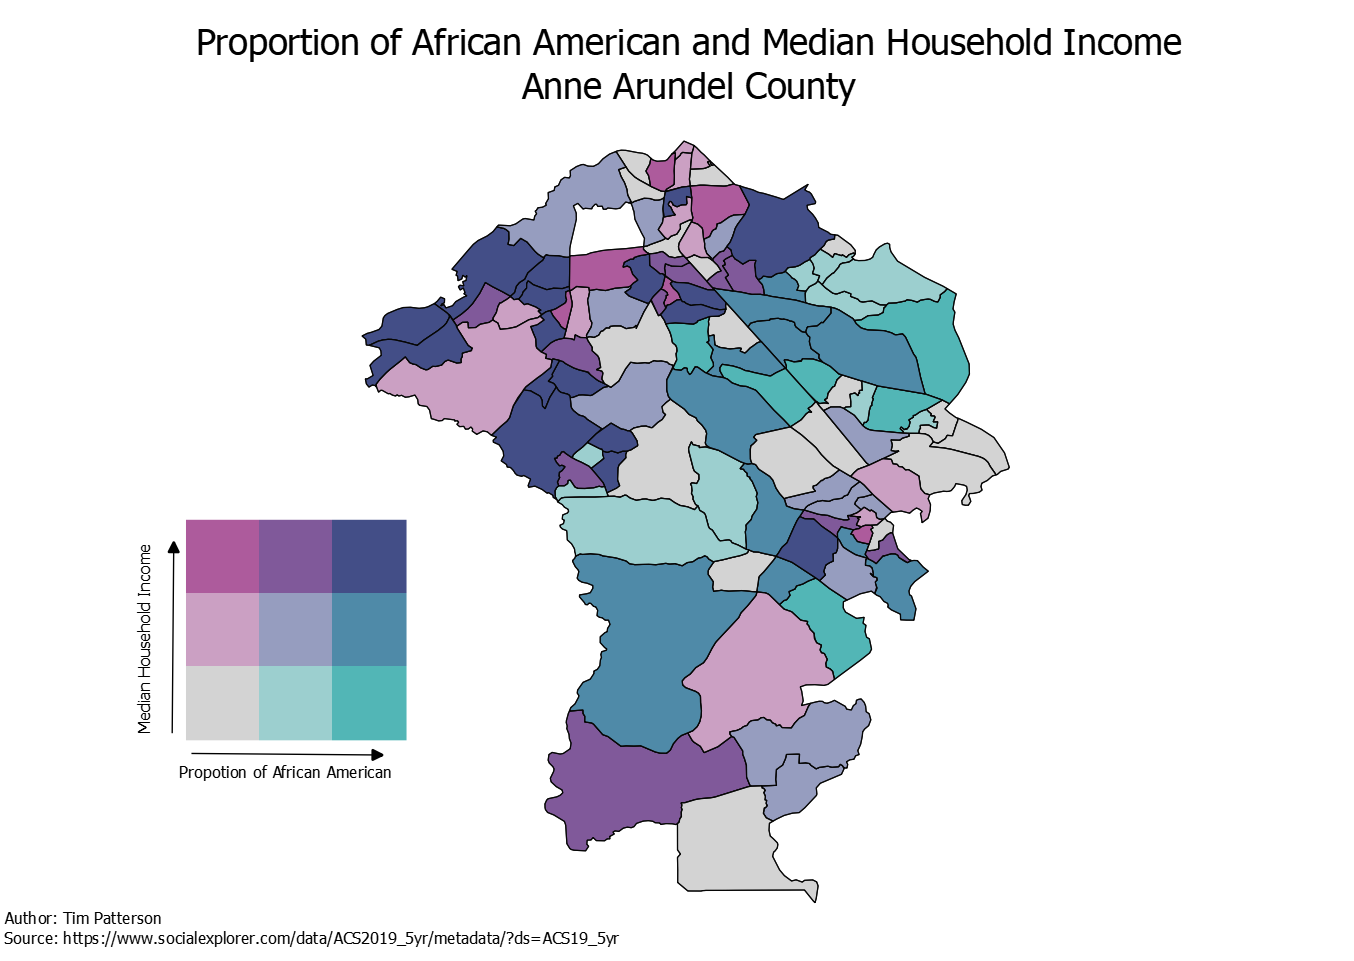
\includegraphics[width=18.81in]{C:/Users/vival/Documents/GES 486/Lab8/Patterson_AAcounty}

\textbf{10. Use qgis2web and put a link here to your github site with
the webmap of your bivariate map. (3 points)}

\url{https://github.com/timpatt1/timpatt1.github.io/tree/master/Patterson_Lab9/qgis2web_2021_05_03-20_50_13_088985}

\hypertarget{reflection-3-points}{%
\subsection{3. Reflection (3 points)}\label{reflection-3-points}}

From this assignment I have gained a better understanding of how the
organization of data is detrimental in the work flow process. Taking the
time to label code chunks as well as leaving comments allows for you to
look back at your code and use it more efficiently in the future. I
struggled with that I would like to remember for this assignment is
editing specific data within a map. The process of transforming specific
data in order to drop and generate variables was very beneficial it
allowed me to better edit my map and highlight specific areas of
interest. This is something I plan to use for projects in the future.

\hypertarget{extra-credit-2-points}{%
\subsection{4. Extra Credit (2 points)}\label{extra-credit-2-points}}

\textbf{Put an image as a legend in your web map.}

Knit your document to a .html file. Submit this knitted document.

\end{document}
